%
% problemstellung.tex -- Beispiel-File für die Beschreibung des Problems
%
% (c) 2020 Prof Dr Andreas Müller, Hochschule Rapperswil
%
\section{Problemstellung
\label{taylor:section:problemstellung}}
Um die numerische Approximation an einem konkreten Beispiel zeigen zu können wird hier die logistische Differentialgleichung \eqref{taylor:section:logistifunction} analysiert.
Es handelt sich hierbei um eine begrenze Wachstumsfunktion. 
Mit dieser Differentialgleichung können zum Beispiel der Verlauf einer Krankheit, der Lebenszyklus eines Produktes oder auch Zerfallsprozesse beschrieben werden. Die Parameter der logistischen Funktion

\begin{equation}
	y'
	=
	k\cdot y(L-y)
	\label{taylor:section:logistifunction}
\end{equation}

sind: $L$ = Endwert und $k$ = Wachstumsrate.
Wir normieren den Endwert $L$ auf 1. Als Anfangswert der Differentialgleichung verwenden wir $y(0)=0.5$.
Der Endwert entspricht zum Beispiel der Anzahl Infizierten am Ende einer Epidemie.
In der Abbildung ~\ref{taylor:section:fig:DGLDarstellung} ist zu erkennen, dass der Wachstumsfaktor $k$ bestimmt, wie steil die Funktion wird.
Somit haben wir nun ein Feld gegeben, indem wir in jedem möglichen Punkt der Funktion eine genau definierte Steigung, bzw. ein genau definiertes $k$ haben.
Um aber das $k$ und damit die Lösung der Differentialgleichung bestimmen zu können müssten wir diese aufwendig ausrechnen.
Deshalb macht es in einem solchen Fall Sinn die Funktion mit kleinen Schritten zu erarbeiten.

\begin{figure}
	\centering
	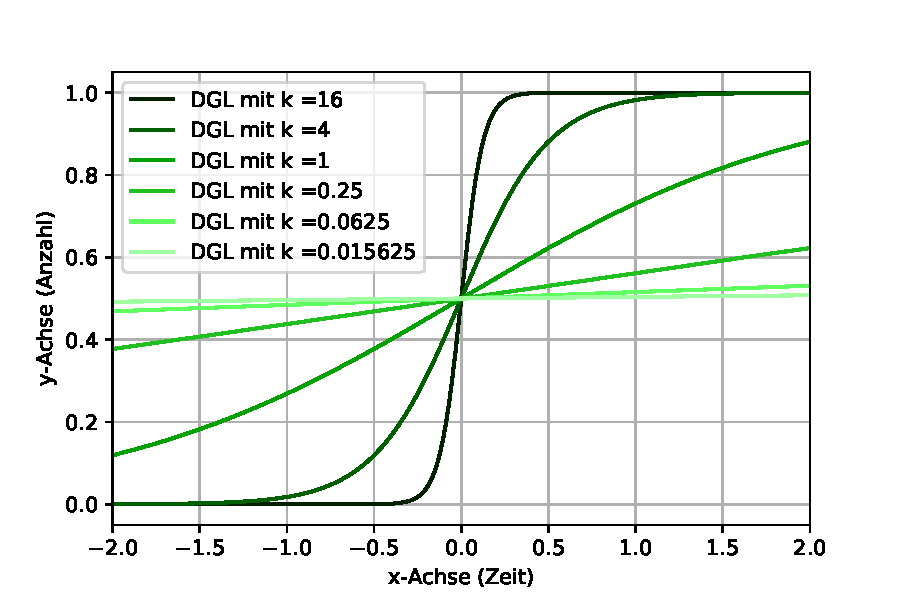
\includegraphics[width=12cm]{papers/taylor/taylorPictures/DGLDarstellung.pdf}
	\caption{Logistische Funktion in Abhängigkeit von k}
	\label{taylor:section:fig:DGLDarstellung}
\end{figure}

Da wir für die Taylor Approximation die Ableitungen bis zur $n$-ten Ordnung benötigen, müssen diese natürlich bekannt sein. Man erhält die Gleichungen

\begin{equation}
	\begin{aligned}
		y'&=k\cdot (y-y^{2})\\
		y''&=k\cdot (y'-2y'\cdot y)\\
		y'''&=k\cdot (y''-2y''\cdot y+y'^{2})\\
		y''''&=k\cdot (y'''-2y'''\cdot y+3y''\cdot y')\\
		y'''''&=k\cdot (y''''-2y'''\cdot y+4y''\cdot y'+3y''^{2})\\
	\end{aligned}
\end{equation}
indem man die logistische Funktion ableitet.

Wie in Abbildung \ref{taylor:section:fig:DGLDarstellung} nun ersichtlich ist, kann jedem möglichen Punkt der logistischen Funktion ein Wachstumsfaktor $k$ zugeordnet werden. Dieser Wachstumsfaktor
\begin{equation}
	k=\frac{-\ln{(\frac{1}{y}-1)}}{x}
\end{equation}
ist also sowohl von $y$ als auch von $x$ abhängig.

\section{Das Taylor Verfahren}
\label{taylor:subsection:Vorgehen}
Die allgemeine Formel der Einschritttheorie sieht so aus:
\begin{equation}
y(x+h) = y(x) + h\cdot f(x,y)
\end{equation}
wobei die Funktin f(x,y) der Approximationsfunktion entspricht mit welcher der nächste Punkt berechnet wird.

Beim Taylor Verfahren soll nun also mit kleinen Schritten der Verlauf der Funktion ausgehend von einem Anfangswert ermittelt werden.
Die Taylor-Reihe
\begin{equation}
f_{T}(x,a)
=
\sum_{n=0}^{\infty}{\frac{f^{(n)}\cdot a}{n!}}\cdot (x-a)^{n}
\label{taylor:section:taylor}
\end{equation}
%$f_{T}(x,a)$ = Taylor Funktion
setzt sich zusammen aus der korrekten Gewichtung der Ableitungen bis zur gewünschten Ordnung.
Je höher der Grad der Auswertung, desto grösser ist der Bereich um den Auswertungspunkt in welchem die Taylor Approximation mit der tatsächlichen Funktion übereinstimmt.
Am Auswertungspunkt wird nun die Taylorfunktion genommen als Approximation der Differentialgleichung um zum nächsten Punkt zu gelangen.
Dieses Verfahren

\begin{equation}
y(x+h)
=
\sum_{n=0}^{g}{\frac{f^{(n)}\cdot h}{n!}}\cdot (x-h)^{n}
\label{taylor:section:taylorapproximation}
\end{equation}

nennt man nun das Taylor Approximationsverfahren.
Dort werden erneut die Ableitungen ausgerechnet und eine weitere Approximationsfunktion aufgestellt, mit der dann der darauf folgende Punkt bestimmen wird.
Je kleiner nun die Schrittweite gewählt wird, desto weniger spielen höhere Ableitungen, beziehungsweise höhere Frequenzanteile, eine Rolle.
In der Abbildung~\ref{taylor:section:fig:LogisticFunctionApproximation} sieht man ein Vergleich des Runge-Kutta Verfahrens und des Taylor Verfahrens.

\begin{figure}
	\begin{center}
	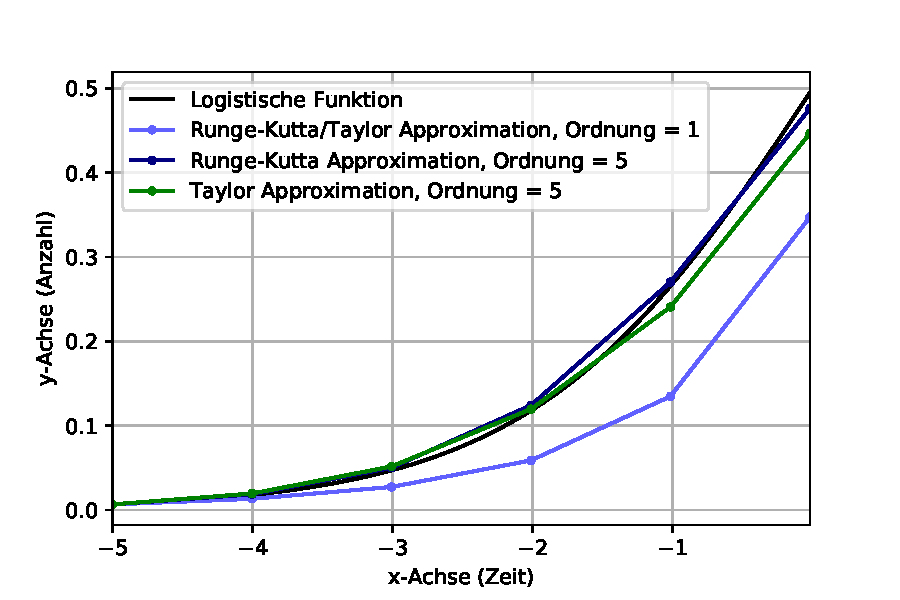
\includegraphics[width=12cm]{papers/taylor/taylorPictures/LogisticFunction.pdf}
	\caption{Gleichung und Approximationen der Logistische Funktion für $k=1$, Approximationen mit 5 Schritten von $-5$ bis $-0.02$ und Startwert der selbe wie bei $k=1$}
	\label{taylor:section:fig:LogisticFunctionApproximation}
	\end{center}
\end{figure}

\begin{table}
\begin{tabular}[h]{|l|l|l|l|l|l|}
	\hline
	Runge-Kutta & $k = 1$ & $k = 2$ & $k = 3$ & $k = 4$ & $k = 5$\\
	\hline
	$n = 1$ & 0.45519 & 0.31990 & 0.11077 & 4.68470e-2 & 6.19930e-2\\
	\hline
	$n = 2$ & 0.38755 & 3.85299e-2 & 5.97521e-2 & 1.05400e-2 & 4.07133e-2\\
	\hline
	$n = 5$ & 0.14751 & 2.39004e-2 & 2.59349e-2 & 1.33486e-2 & 1.88327e-2\\
	\hline
	$n = 10$ & 6.88690e-2 & 4.37589e-3 & 4.37432e-3 & 2.58736e-3 & 3.50711e-3\\
	\hline
	$n = 1000$ & 6.19312e-4 & 5.23506e-7 & 1.84704e-07 & 1.85763e-7 & 1.85765e-07\\
	\hline
	$n = 100000$ & 6.18453e-6 & $5.13468\cdot 10^{-11}$ & $1.96497\cdot 10^{-11}$ & $1.96507\cdot 10^{-11}$ & $1.96507\cdot 10^{-11}$\\
	\hline
\end{tabular}

\caption{$k$ = Ordnung, $n$ = Schritte, Start = $-5$, Ende = $-0.02$, (letzte Ziffer abgerundet)}
\end{table}

\begin{table}
\begin{tabular}[h]{|l|l|l|l|l|l|}
	\hline
	Taylor & $k = 1$ & $k = 2$ & $k = 3$ & $k = 4$ & $k = 5$\\
	\hline
	$n = 1$ & 0.45519 & 0.27840 & 0.27948 & 0.29078 & 0.29515\\
	\hline
	$n = 2$ & 0.38755 & 0.20040 & 0.19400 & 0.19579 & 0.19663\\
	\hline
	$n = 5$ & 0.14751 & 5.30816e-2 & 4.80256e-2 & 4.79241e-2 & 4.79851e-2\\
	\hline
	$n = 10$ & 6.88690e-2 & 1.60657e-2 & 1.38830e-2 & 1.38673e-2 & 1.38751e-2\\
	\hline
	$n = 1000$ & 6.19312e-4 & 2.11126e-6 & 1.90164e-6 & 1.90183e-6 & 1.90183e-6\\
	\hline
	$n = 100000$ & 6.18453e-6 & 2.10965e-10 & 1.90226e-10 & 1.90226e-10 & 1.90226e-10\\
	\hline
\end{tabular}

\caption{$k$ = Ordnung, $n$ = Schritte, Start = $-5$, Ende = $-0.02$, (letzte Ziffer abgerundet)}
\end{table}

\begin{figure}
	\centering
	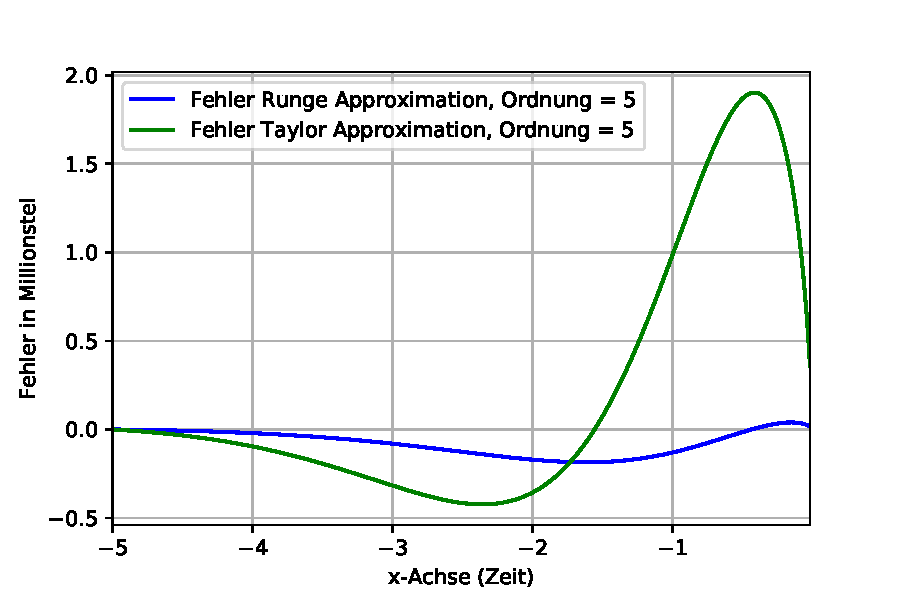
\includegraphics[width=12cm]{papers/taylor/taylorPictures/FehlerRungeUndTaylor.pdf}
	\caption{Fehler der Approximationen bei 1000 Schritten von $-5$ bis $-0.02$ und Startwert der selbe wie bei $k=1$}
	\label{taylor:section:fig:FehlerRungeTaylor}
\end{figure}

\subsection{Auswertung des Vergleiches}
\label{taylor:subsection:Auswertung}
Die ersten Spalten der beiden Verfahren sehen gleich aus, weil die Approximationen erster Ordnung auf das selbe herauskommen, nämlich auf das Approximieren der Funktion mit geraden erster Ordnung, was der Steigung im Auswertungspunkt entspricht.

Beim Punkt $n=1$ und $k=2$ ist die Taylor Approximation besser als Runge-Kutta.
Eine Approximation mit dem Grad 2 und einem Schritt über eine sich so stark verändernde Kurve ist aber eher ein Glückstreffer als ein mathematischer Erfolg.
Im Allgemeinen kann gesagt werden dass das Runge-Kutta Verfahren in diesem Fall ein kleineren Fehler aufweist. Dies ist auch in der Abbildung \ref{taylor:section:fig:FehlerRungeTaylor} zu sehen.

\section{Probleme mit der Logistischen Funktion}
\label{taylor:subsection:Probleme}
Die logistische Funktion wurde gewählt, weil es eine anschauliche, nichtlineare Differentialgleichung ist welche sich somit gut eignet um das Runge-Kutta Verfahren mit dem Taylor Verfahren zu vergleichen.
Dabei traten allerdings folgende zwei Probleme auf.

\subsection{Konvergenz}
\label{taylor:subsection:Konvergenz}
Wie in Abbildung 
\ref{taylor:section:fig:DGLDarstellung}
ersichtlich ist, läuft die Differentialgleichung im Punkt 0 gegen 0.5 und bei $\infty$ gegen 1.
Wird nun also diese Differentialgleichung approximiert, dann ist sowieso klar auf welchem Wert wir ungefähr landen werden.
Um eine aussagekräftige Antwort auf die Frage der Qualität geben zu können wurden die Fehler über den ganzen Verlauf der Approximation verglichen. Siehe dazu Abbildung \ref{taylor:section:fig:FehlerRungeTaylor}.

\subsection{Gefähliche Umgebung des 0-Punktes}
\label{taylor:subsection:0Punkt}
Wie in Abbildung 
\ref{taylor:section:fig:DGLDarstellung}
klar dargestellt ist, ist die Ableitung in direkter Umgebung vom Punkt (0, 0.5) zwischen 0 und $\infty$.
Wenn also eine Approximation der Differentialgleichung durch diesen Punkt geht, wird sie durch einen auch noch so kleinen Fehler eine ganz andere Ableitung berechnen und somit völlig anders verlaufen.
Um dies zu umgehen wurde einfach nicht durch diesen Wendepunkt gegangen, sondern nur bis 0.02 davor.
Man könnte nun aber die erhaltenen linke Kurve an dem Wendepunkt punktspiegeln und hätte so die zweite Hälfte ebenfalls, welche somit sowieso redundant und für uns nicht intressant ist.

%\nameref
%\pageref{}
%\numref
%\ref{taylor:section:loesung}.
%\ref{taylor:section:folgerung}.


